%\documentclass[pdf,final]{prosper}
\documentclass[pdf,final,norman]{prosper}

\title{Data models in the VO: how do they make code better?}
\newcommand{\at}[1]{}
\author{Norman Gray\at{Starlink/University of Glasgow},
        David L Giaretta\at{Starlink/RAL},
        David Berry\at{Starlink/University of Central Lancashire},
        Malcolm Currie\at{Starlink/RAL}, 
        Mark Taylor\at{Starlink/University of Bristol}}

%\title{Data modelling, data access, and code}
%\author{Norman Gray}
\institution{Starlink @ \{Glasgow, RAL, Central Lancashire, RAL,
Bristol\}, UK}
\slideCaption{Norman Gray, www.starlink.ac.uk / ADASS XIII,
Strasbourg, 2003 October 14}
%\Logo{\vbox{\hsize=1.2cm \parindent=0pt \parskip=0pt \nointerlineskip
%        \hbox to \hsize{\hss\includegraphics[width=\hsize]{starlink_logo1.eps}}
%        \hbox to \hsize{\hss\includegraphics[width=\hsize]{GUVI.eps}}
%        }}
\Logo{\vbox{\hsize=1.2cm \parindent=0pt \parskip=0pt \nointerlineskip
        \hbox to \hsize{\hss
\includegraphics[width=\hsize]{starlink_logo_aa.eps}}
%        \hbox to \hsize{\hss\includegraphics[width=\hsize]{starlink_logo1.eps}}
%        \hbox to \hsize{\hss\includegraphics[width=\hsize]{GUVI.eps}}
        }}

\usepackage{times}
\usepackage{graphicx}
\usepackage{url}
\usepackage{myprosper}

\newenvironment{myslide}[1]{\begin{slide}{#1}\slidetoc{#1}}{\end{slide}}

\makeatletter
\def\verbatim@font{\fontsize{7}{8}\selectfont\ttfamily}
\makeatother
%\def\UrlFont{\fontsize{10}{11}\selectfont\ttfamily}


\begin{document}

\maketitle

\begin{slide}{Overview}
\tableofslides
\end{slide}



\begin{slidegroup}{models}{Why do we need models?}

\begin{myslide}{What are data models?}

\begin{itemize}

\item Data Models exist in people's heads.

\item Data modelling consists of making these explicit on paper.

\item How many models?

\item Which model does the user/system want?
%, so that (a) we can discover if there is more
%than one important model, and (b) we can develop using the model which
%has the best impedance match with the community being targeted.

\item Thus
modelling is not just about communications -- about bits (or angle
brackets!) on the wire -- but is a software quality and usability
issue.

\end{itemize}
\end{myslide}


\begin{myslide}{Languages}
\includegraphics[width=\hsize]{models.eps}
\end{myslide}

\begin{myslide}{Languages}
\vbox to 0pt{\hbox to \hsize{\hss\includegraphics[width=0.5\hsize]{models.eps}}\vss}
\begin{itemize}
\item interface${}={}$`language'
\item \dots and thus a model
\item Systems are modelled
\item Users create models
\item \dots by reading documentation and language
\item If the three match, we get usable/correct/fast code
\item If not, not
\end{itemize}
Aren't mismatches inevitable?  What do a star and a database record
have in common except a tendency to generate entropy?
\end{myslide}

\begin{myslide}{Models are for thinking with}
\begin{itemize}
\item A data model is the set of primitive concepts that we hope our user
thinks with,
\item \dots the language expresses,
\item \dots and the underlying system implements.
\end{itemize}
If the model is made explicit at the beginning of the process, then we
can think with it, check it is consistent, both with itself and with
the outside world.
\end{myslide}

\begin{myslide}{So how do we make it explicit?}
\begin{itemize}
\item Obvious answers are XSchema, UML, Java class library.
\item But these come with a lot of extra baggage, which worms its way
into the model (do stars \emph{really} have methods?).
\item (If we think about syntax too early, we end up modelling the
syntax.)
\item So either decide that you \emph{want} the baggage, or use a more
modelling language which describes things at a more primitive level.
\end{itemize}
\end{myslide}

% 
% \section{Language, models and usability}
% 
% In linguistics, the well-known Sapir-Whorf hypothesis states that the
% way we conceive of the world depends on the language we use to
% describe it.  Or more compactly, we can only think what we can
% say.
% 
% This matters to us, since when we create software systems, we are
% often creating a `language' -- in a user-interface, an API or a
% protocol -- which users must employ to interact with an underlying
% system, be it an application, a library, or a remote service (here and
% below, we use the term `users' to apply both to astronomers using a
% mouse and programmers using an API or protocol).  If there is a good
% three-way match between the concepts in the user's head, the concepts
% implied by the language, and the concepts implicit in (some aspect of)
% the system's actual design, then the user's interactions with the
% system will be straightforward and largely error-free.  If there is a
% mismatch, they will not.  This is not just a matter of user-interface
% design; if the `user' is a programmer working with an API or a
% protocol, then this three-way match will help them write correct code
% faster, and produce an application which will in turn be usable by its
% eventual audience.
% 
% We can all think of systems which fail to exhibit this full match, but
% in some cases, surely a mismatch is inevitable.  After all, a star and
% a database record surely have nothing in common except a tendency to
% generate entropy.  This is why we need a data model.
% 
% A data model is the set of primitive concepts that we hope our user
% thinks with, the language expresses, and the underlying system
% implements; it is the rendezvous which helps the system as a whole
% hang together.  If the model is made explicit during the development
% process, then it can itself be examined, criticised, and checked for
% consistency with itself and with the external system it is
% supposed to model, whether that is, say, CDS or `a quantity'.  Once
% the model is itself part of the language of development, we can think
% with it, and talk about it, rather than merely mumble.
% 
% This immediately prompts the question of just how we make the model
% explicit.  There are several obvious answers to this, of which the
% most currently fashionable will be XSchema, UML, and `a Java
% class library'.  The problem with each of these is that they each come with
% far too much baggage.  This is another aspect of the Sapir-Whorf
% hypothesis: we tend to see the world in terms of the
% structure of the language we use to describe it.  That means that if
% we use XSchemas to model the world, we will discover that the world is
% made of things enclosing other things, with attributes, and if we use an O-O language,
% the world turns out to have methods.  That is, our choice of modelling
% language biases our model to have certain features, \emph{irrespective} of
% whether these features are present in the system being modelled.
% 
% A separate problem is to start thinking about syntactical or
% presentational details too early.  If we retrofit a data model, it
% will end up being a poor model of the world, but an excellent
% model of our syntax.
% % During the UCD modelling effort, we found ourselves asking questions
% % which purported to be about astronomy, but which were really about
% % underscores.
% 
% There are two strategies to deal with this.  The first is to embrace
% the problem, acknowledge that our choice of language is not neutral,
% and make sure that choice is a good one.  The second is to choose a
% more primitive modelling language, which will push fewer things into
% the model.  We will return to this question in section~\ref{s:techniques}.


\end{slidegroup}


\begin{slidegroup}{votable}{VOTable and other models}

\begin{myslide}{VOTable}
Viewed as a way of\dots
\begin{itemize}
\item \dots transporting catalogues from catalogue producers to catalogue
consumers,
\item \dots encoding \emph{all} available information about a
catalogue or image
\end{itemize}
\dots VOTable is excellent.  There's a good match here between system,
language and user.

VOTable is expressive, recursive, and flexible.  \emph{But\dots}. 
\end{myslide}

\begin{myslide}{VOTable II}
\dots it's expressive, recursive, and flexible.

These are \emph{good} things if you're an archivist.  But \emph{bad}
things if all you want is an image.  So:
\begin{itemize}
\item extend VOTable?  \emph{No!}: that would just make it more complicated.
\item simplify VOTable$\to$ miniVOTable?  No: that limits the
flexibility without really addressing the problem.
\item provide libraries?  Yeeesss\dots
\end{itemize}
The problem is not with VOTable; instead there's \emph{more than one
model}, because there's more than one constituency of users (ie,
programmers professional and casual).
\end{myslide}

\begin{myslide}{VOTable III}
\vbox to 0pt{\hbox to \hsize{\hss\includegraphics[width=0.5\hsize]{models.eps}}\vss}
\begin{itemize}
\item \begin{minipage}{0.5\hsize}
      \raggedright
      Data consumers (query agent, programmer) have a simple-minded model.
      \end{minipage}
\item \begin{minipage}{0.5\hsize}
      \raggedright
      Because there's multiple models, we
      don't have the three-way match any more; so lower software
      quality.
      \end{minipage}
\item Step 1: identify and express the data consumer's model
\item Step 2: \emph{then} work out how to map one model to the other
in principle, at the system end
\item Step 3: \emph{then} choose syntax/technology
\end{itemize}
\end{myslide}

\end{slidegroup}

% We contend that there is in fact more than one model relevant to the
% VO, and that while the VOTable model is an excellent and valuable fit
% to the archivists' model of data, it may be a poor match for many
% users or (which is much the same thing) for the software written to
% service the sort of end-user astronomical applications which the VO
% targets.



\begin{slidegroup}{tech}{Modelling technologies}

% Modelling work in other areas shows the importance of abstraction in
% the concrete goal of freeing software design from the particulars of
% any single implementation. This is extremely important for the VO
% because it allows us, and the software we write, to deal with the
% essentials of the data rather than the superficial aspects of a
% particular format such as XML or FITS. We discuss the work that we and
% others have been doing within this context; with this in mind, we will
% also review some of the various modelling languages available, such as
% XSchemas, UML, OMG MDA, HUTN, RDF, and Topic Maps.
% \end{abstract}

\begin{myslide}{XSchema}
\begin{itemize}
\item Well-known: XML instance syntax
\item Verbose
\item Complicated
\item Elaborate type system, looks familiar to database people; also this
is the type system used by other W3C standards
\item Langauges like RelaxNG have easier-to-read syntax and can
translate back-and-forth to XSchema
\item Not really a modelling language, but modelling is involved in
writing a schema
\end{itemize}
\end{myslide}

\begin{myslide}{UML}
\begin{itemize}
\item For designing object-oriented libraries
\item \dots thus usable for general modelling
\end{itemize}
\end{myslide}

\begin{myslide}{RDF and OWL}
\begin{itemize}
\item Set of primitive ideas for representing relations between
entities -- subject-predicate-object
\item Base RDF is mostly concerned with syntax
\item OWL (Ontology Language for the Web) supplements RDF with
properties such as \texttt{minCardinality}, \texttt{equivalentClass}
and \texttt{intersectionOf} which support basic reasoning
\item Notation3 is \emph{much} more readable than ugly RDF/XML: for example
\texttt{\#apple :obs.mass "200g" .}
\end{itemize}
\url{http://www.astro.gla.ac.uk/users/norman/note/2003/rdf-intro/}
\end{myslide}

\begin{myslide}{Other modelling languages}
\begin{itemize}
% HUTN <http://www.dstc.edu.au/Research/Projects/Pegamento/hutn/>
% OMG MDA at <http://www.omg.org/mda/>
% OMG XMI at <http://www.omg.org/technology/documents/formal/xmi.htm>
\item XMI (XML Metadata Interchange): XML-based modelling language
intended to help generate and exchange mutually consistent XSchemas,
UML and code (CORBA and IDL interfaces).
\item HUTN (Human-Usable Textual Notations): how to write XMI without
angle-brackets.
\item MDA (Model Driven Architecture): ties these together.
\end{itemize}
Buzzzzzzzz.
\end{myslide}

\end{slidegroup}


\end{document}
